
\documentclass[12pt, a4paper]{article}
\usepackage[utf8]{inputenc}
\usepackage{a4wide}
\usepackage{color, amssymb}
\usepackage[margin=2.5cm]{geometry}
\usepackage{listings, amsmath, float}
\renewcommand{\baselinestretch}{1.5}
\setlength\parindent{24pt}
\usepackage{graphicx, cancel}
\graphicspath{ {./images/} }

\title{First Project}
\author{Odysseas Stavrou, Olga Tsirou}
\date{October 2020} 

\begin{document}
\noindent\rule{\textwidth}{1.5pt}

\begin{center}
{\bf Telecommunication Systems I} \\ 
 Report of the 2nd Project\\
 Olga Tsirou 2018030061\\
 Odysseas Stavrou 2018030199\\
 November 2020\\
 Technical University of Crete\\
 Prof.:\ A. P. Liavas 
\end{center}
\noindent\rule{\textwidth}{1.5pt}

\begin{enumerate}
    \item[A.] Spectral Power Density study of PAM signals:
    \begin{enumerate}
        \item[A.1] Creating an orthogonal \(\phi(t)\) and calculating it's PSD.\\
        Code for creating an orthogonal \(\phi(t)\)
        \begin{lstlisting}[language=MATLAB]
[phi, phi_t] = srrc_pulse(T, over, A, a);
phi_F = abs(fftshift(fft(phi,N_FFT).*Ts)).^2;
        \end{lstlisting}
        \begin{figure}[H]
            \centering
            \noindent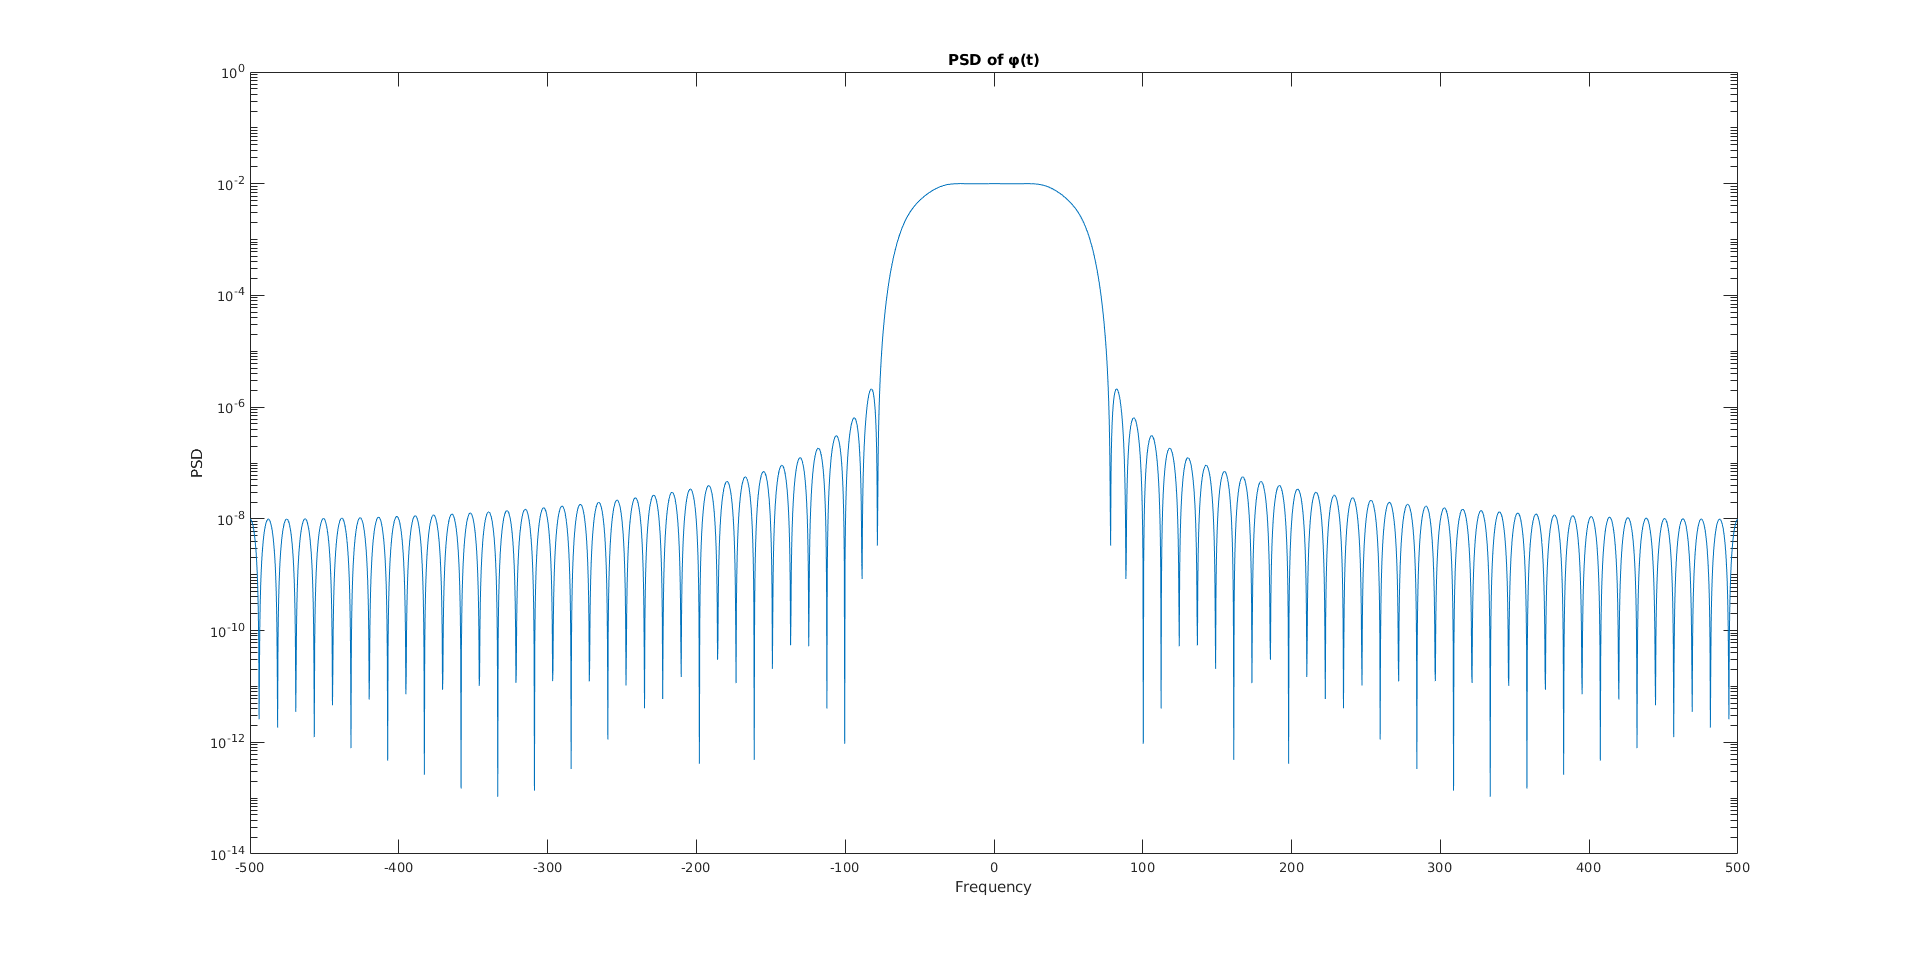
\includegraphics[width=\textwidth]{PHI_PSD.png}
            \caption{Power Spectral Density of \(\phi(t)\)}
        \end{figure}

        \item[A.2] Symbol Creation and carrier modulation using 2-PAM:\\
        Create 100 random bits and represent them in symbols using 2-PAM and the \textbf{modulate\_2PAM} function\\
        Code for creating and modulating a 2-PAM signal \(X(t)\):
        \begin{lstlisting}[language=MATLAB]
[X_t_t,X_t,dur] = modulate_2PAM(phi_t, phi, N_bits, Ts, over);
psd_phi = (1/T).*phi_F;
function [X_t_t, X_t, dur] = modulate_2PAM(t_phi, phi, N_bits, Ts, over)
% generate random bit stream
bit_stream = randi([0 1], 1 , N_bits);
% Symbolize it using 2-PAM
pamed_stream = bits_to_2PAM(bit_stream);
% Upsample it
X_delta = 1/Ts * upsample(pamed_stream,over);
T_delta = 0:Ts:length(X_delta)*Ts - Ts;
% plot(T_delta, X_delta);
% Modulate it with the carrier wave
X_t_t = T_delta(1) + t_phi(1):Ts:T_delta(end) + t_phi(end);
X_t = conv(X_delta, phi) .* Ts;
dur = length(T_delta)*Ts;
end	
    \end{lstlisting}

        \begin{figure}[H]
            \centering
            \noindent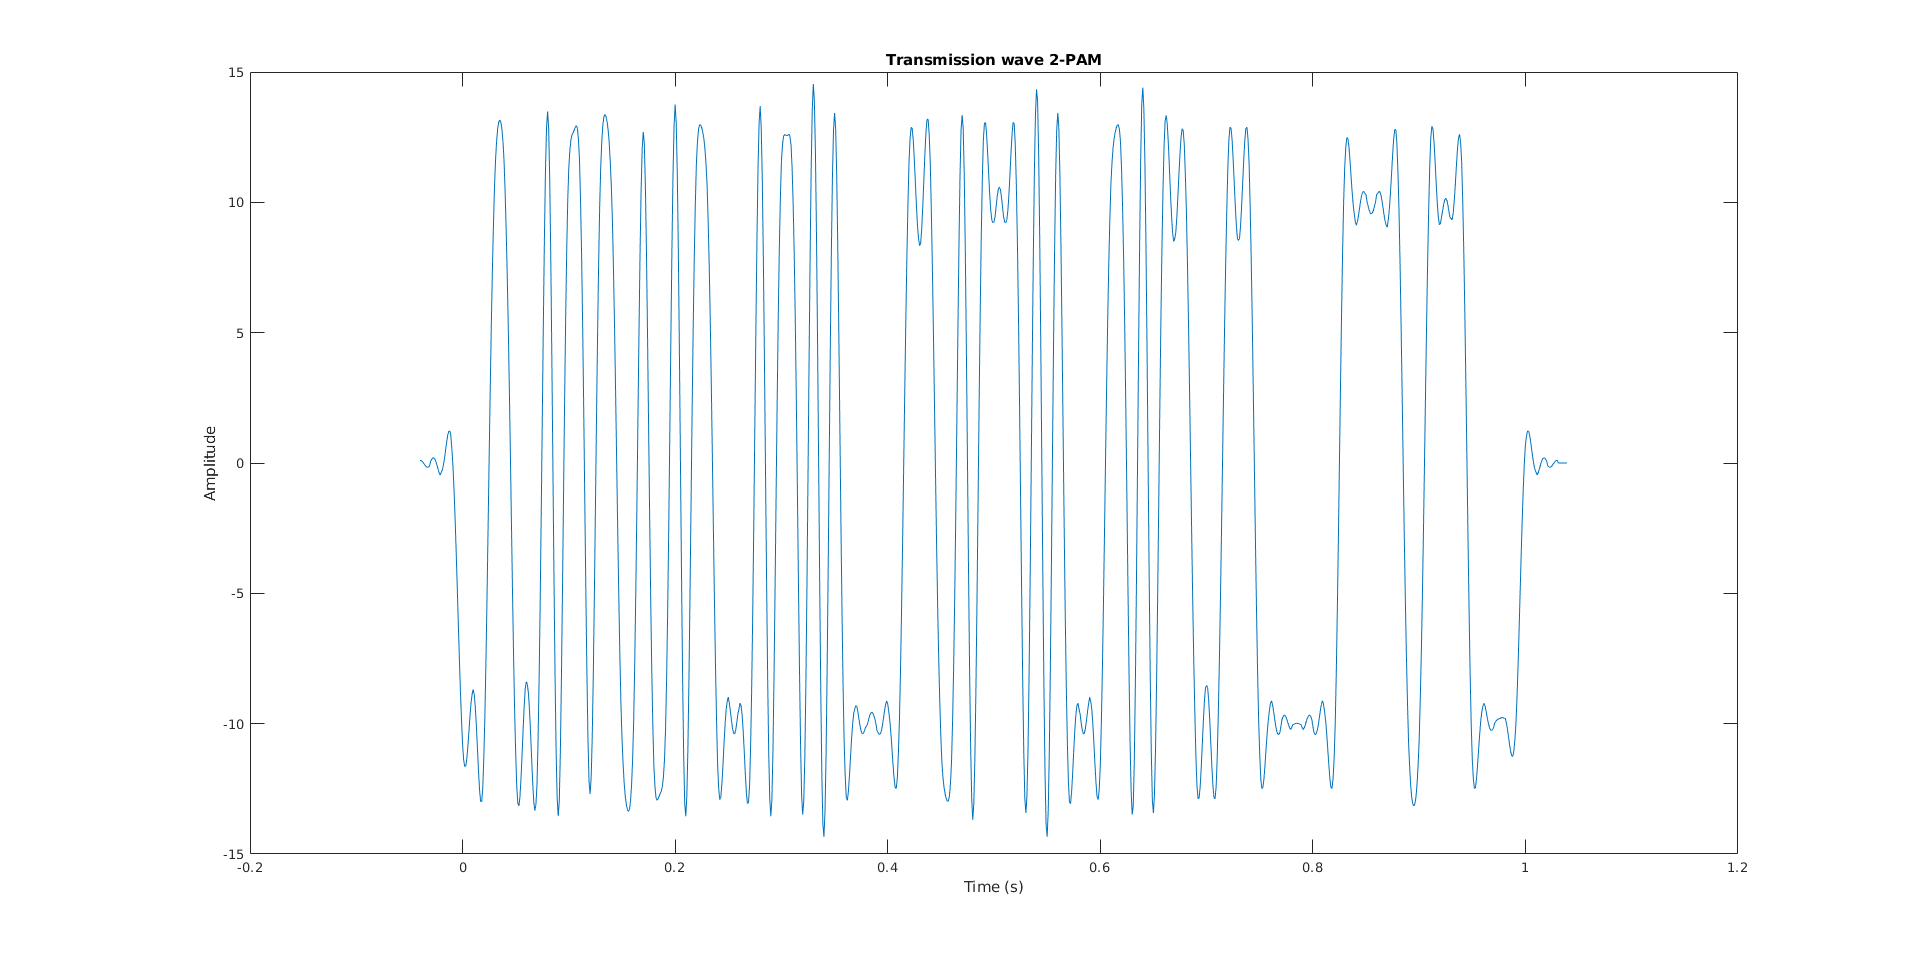
\includegraphics[width=\textwidth]{TX_2PAM.png}
            \caption{Transmission wave containing the modulated symbols}
        \end{figure}
        The PSD of the signal \(X(t)\), when the amount of symbols are infinite, can be calculated as such:
        \[S_X(F) = \frac{\sigma_X^2}{T} |\Phi(F)|^2 \]
        The variance in the above equation can be calculated:
        \[f_{S}(s) = \begin{cases} 
        	\frac{1}{2}, & s = 1 \\
        	\frac{1}{2}, & s = -1 \\
        	0, & \text{otherwise}
        \end{cases}
        \]
        \[E[S] = \sum_{s}sp(s) = (1)\cdot\frac{1}{2} + (-1)\cdot\frac{1}{2} = 0\]
        \[Var(S) = \sum_{s}(s-E[S])^2p(s) = (1 - 0)^2\cdot\frac{1}{2} + (-1 - 0)^2\cdot\frac{1}{2} = 1 \]
        The resulting PSD equation becomes:
        \[S_X(F) = \frac{|\Phi(F)|^2}{T} \]

        \item[A.3] Periodogram of \(X(t)\)\\
        The Periodogram is calculated using the following equation:
        \[P_X(F) = \frac{|F[X(t)]|^2}{T_{total}}\]
        where \(T_{total}\) is the time of \(X(t)\) in seconds\\
        Code for calculating the Periodogram of \(X(t)\)
        \begin{lstlisting}[language=MATLAB]
Pxf = abs(fftshift(fft(X_t, N_FFT).*Ts)).^2/dur;
       	\end{lstlisting}
        \begin{figure}[H]
            \centering
            \noindent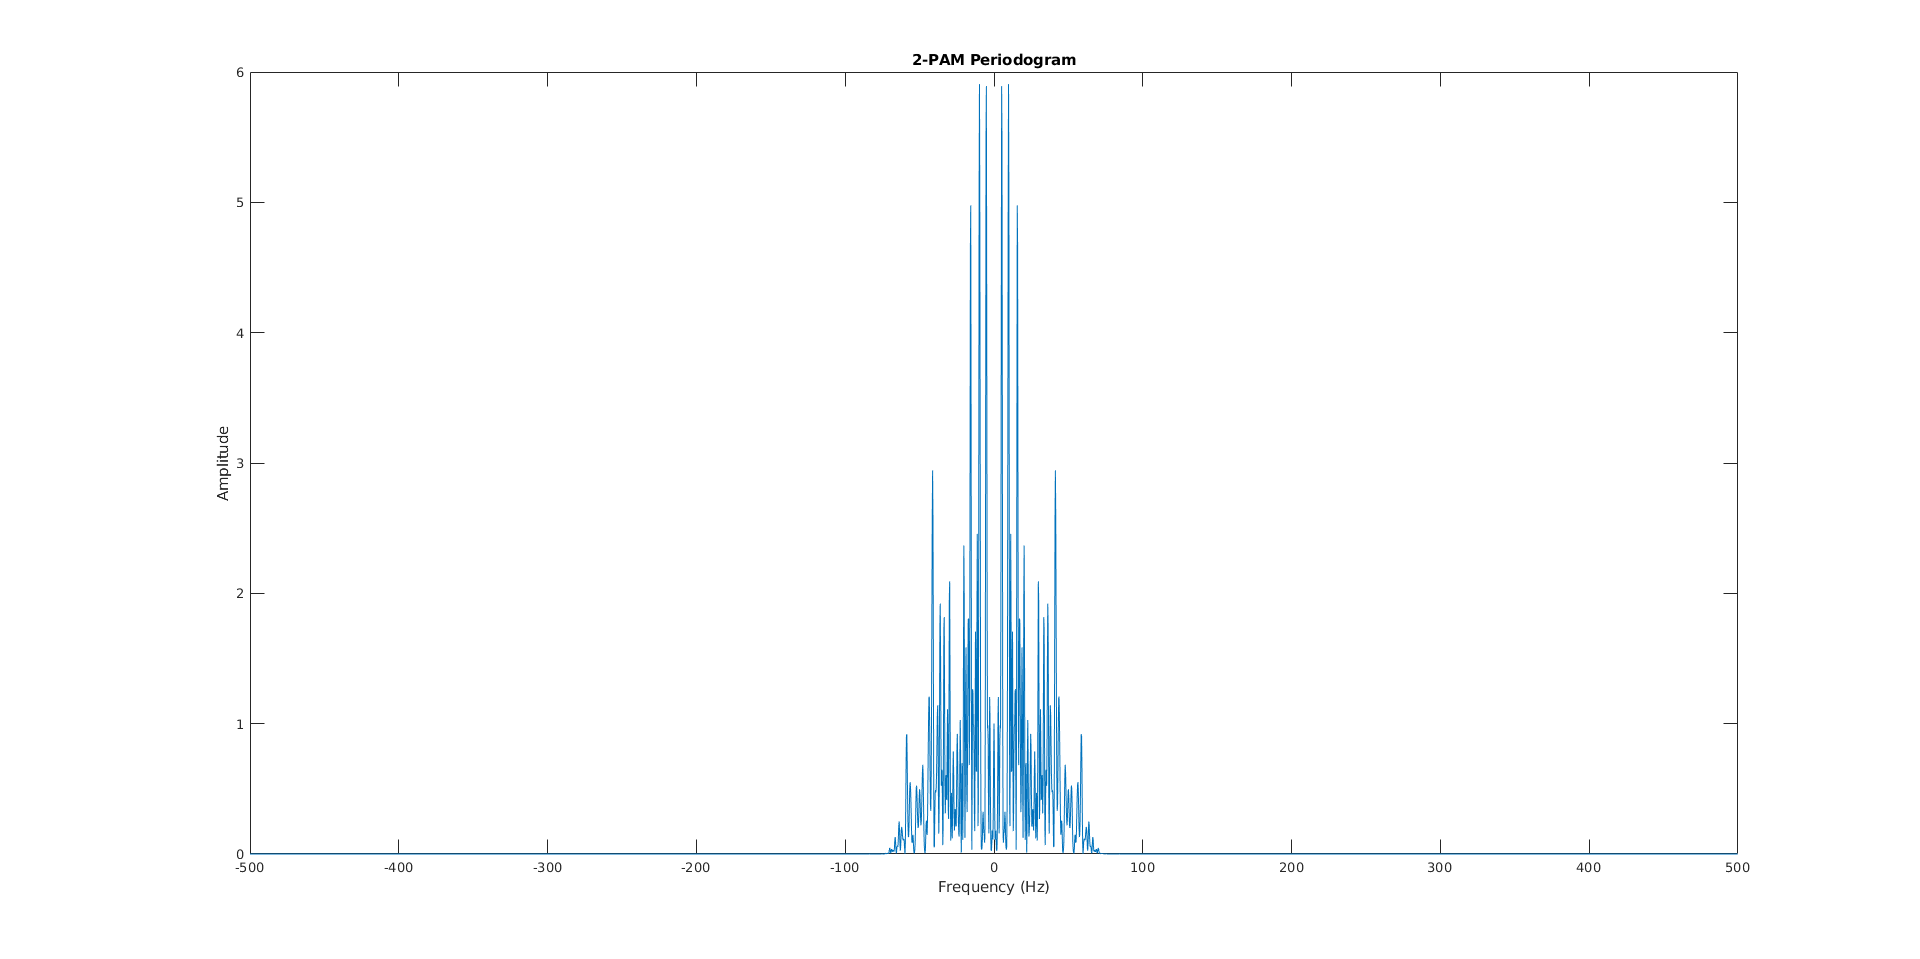
\includegraphics[width=\textwidth]{2PAM_PSD_PLOT.png}
            \noindent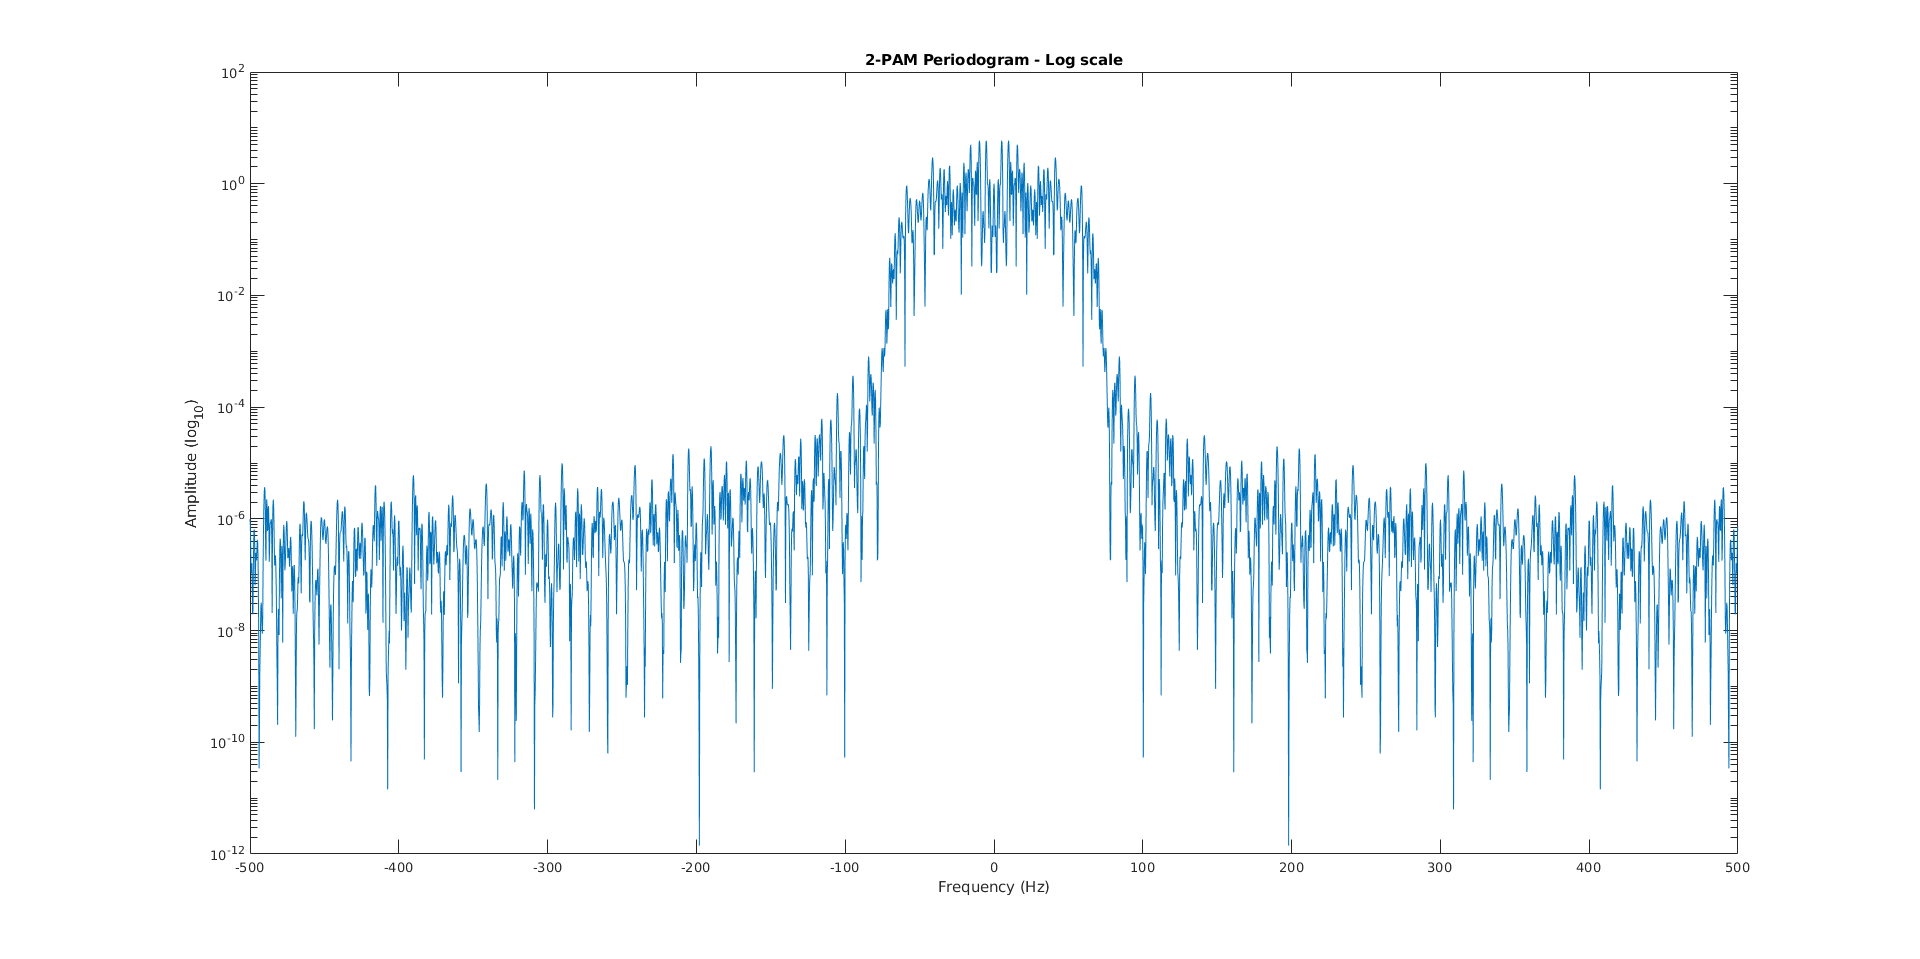
\includegraphics[width=\textwidth]{2PAM_PSD.png}
            \caption{Periodogram of \(X(t)\) in both normal and semilogarithmic axis}
        \end{figure}
        In order to calculate the Estimated PSD we need to take the average values of (in our case 500) Periodograms.\\
        Code for calculating the estimated PSD of \(X(t)\)
        \begin{lstlisting}[language=MATLAB]
for i=1:K
[~,X_t,dur] = modulate_2PAM(phi_t, phi, N_bits, Ts, over);
Pxf_table(i,:) = abs(fftshift(fft(X_t,N_FFT).*Ts)).^2/dur;
end
        \end{lstlisting}
        \begin{figure}[H]
            \centering
            \noindent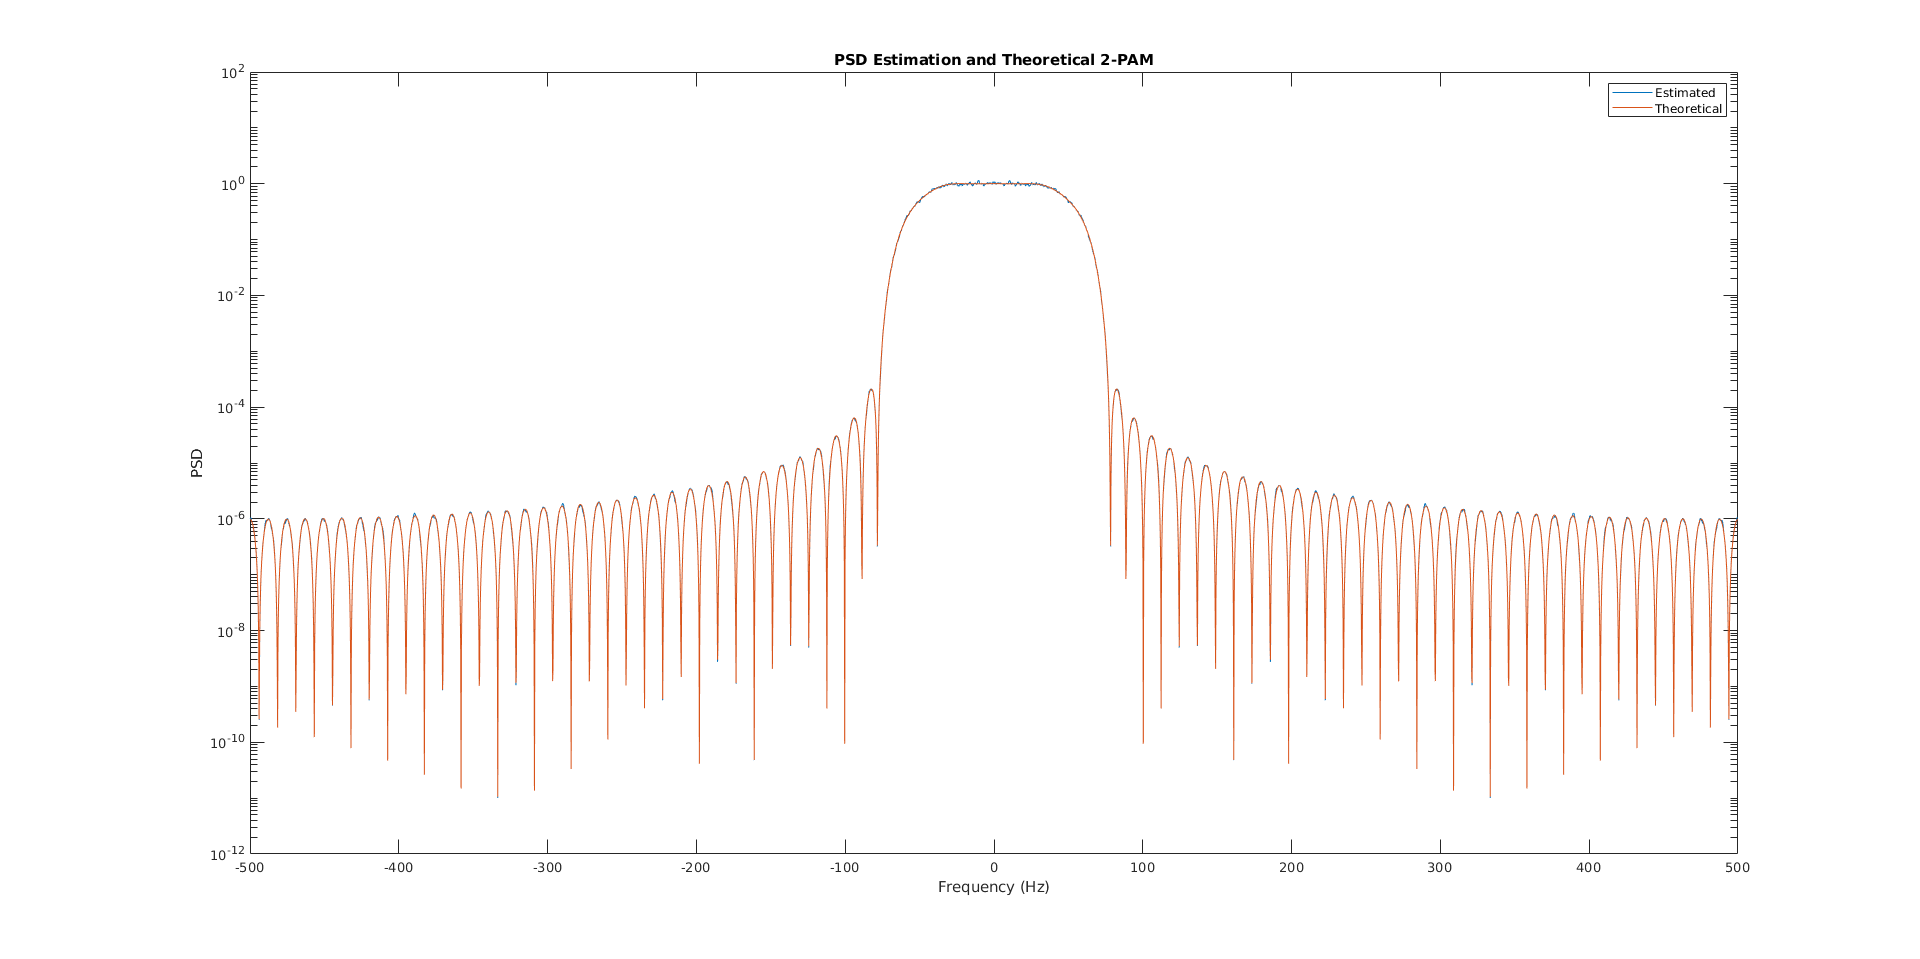
\includegraphics[width=\textwidth]{PSD_EST_THE_2PAM.png}
            \caption{Theoretical and Estimated graphs of the PSD of the signal \(X(t)\) modulated with 2-PAM.\ 
            Small ripples are observed in the estimated graph.}
        \end{figure}

		By increasing the number of loops (K, samples to average) and by increasing the symbols to transmit (N) we can conclude the following:\\
		\begin{itemize}
			\item By increasing K we are getting closer and closer to the theoretical PSD value, because we average more values we are minimizing the deviation from the theoretical value
			\item Increasing N, does not produce a better result, because it does not change the amount of samples that are going to be averaged, it just changes the amount of symbols ought to be transmitted 
		\end{itemize}
        \item[A.4] Symbol Creation and carrier modulation using 4-PAM\\
        Using the same methodology and the corresponding function \textbf{modulate\_4PAM}
        \[f_{S}(s) = \begin{cases} 
        	\frac{1}{4}, & s = 3 \\
        	\frac{1}{4}, & s = 1 \\
        	\frac{1}{4}, & s = -1 \\
        	\frac{1}{4}, & s = -3 \\
        	0, & \text{otherwise}
        \end{cases}
        \]
        \[E[S] = \sum_{s}sp(s) = (3)\cdot\frac{1}{4}+(1)\cdot\frac{1}{4}+(-1)\cdot\frac{1}{4}+(-3)\cdot\frac{1}{4} = 0\]
        \[Var(S) = \sum_{s}(s-E[S]) = 
        (3 - 0)^2 \cdot \frac{1}{4} + (1 - 0)^2 \cdot \frac{1}{4} + (-1 - 0)^2 \cdot \frac{1}{4} + (-3 - 0)^2 \cdot \frac{1}{4}\]
        \[ = \frac{18}{4} + \frac{2}{4}  = 5\]
        The resulting PSD equation becomes:
        \[S_X(F) = \frac{5}{T}|\Phi(F)|^2 \]
        Code for creating and modulating a 4-PAM signal, theoretical and estimated PSD of \(X(t)\):
        \begin{lstlisting}[language=MATLAB]
[X_t_t,X_t,~] = modulate_4PAM(phi_t, phi, N_bits, Ts, over);
for i=1:K
[~,X_t,dur] = modulate_4PAM(phi_t, phi, N_bits, Ts, over);
Pxf_table(i,:) = abs(fftshift(fft(X_t,N_FFT).*Ts)).^2/dur;
end
psd_phi = 5/T.*phi_F;

function [X_t_t, X_t, dur] = modulate_4PAM(t_phi, phi, N_bits, Ts, over)
% generate random bit stream
bit_stream = randi([0 1], 1 , N_bits);
% Symbolize it using 2-PAM
pamed_stream = bits_to_4PAM(bit_stream);
% Upsample it
X_delta = 1/Ts * upsample(pamed_stream,over);
T_delta = 0:Ts:length(X_delta)*Ts - Ts;
% Modulate it with the carrier wave
X_t_t = T_delta(1) + t_phi(1):Ts:T_delta(end) + t_phi(end);
X_t = conv(X_delta, phi) .* Ts;
dur = length(T_delta)*Ts;
end
        \end{lstlisting}
        \begin{figure}[H]
            \centering
            \noindent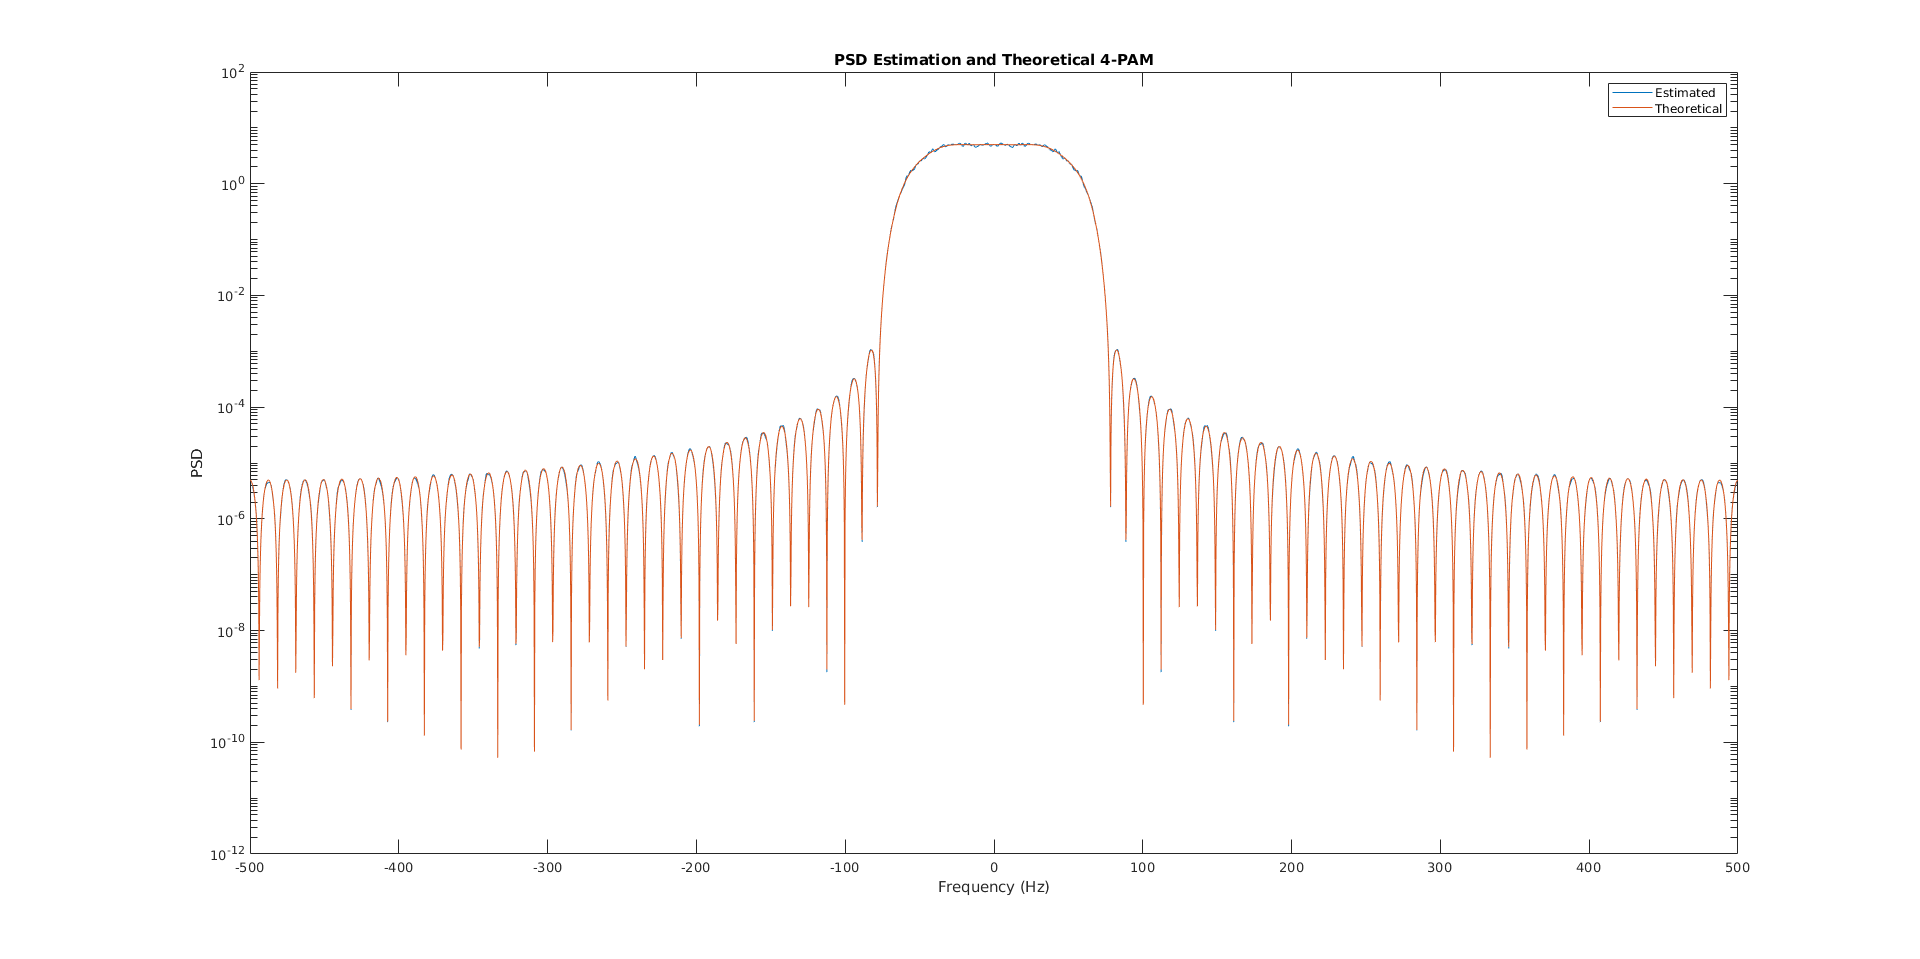
\includegraphics[width=\textwidth]{PSD_EST_THE_4PAM.png}
            \caption{Theoretical and Estimated graphs of the PSD of the signal \(X(t)\) modulated with 4-PAM.\
            Small ripples are observed in the estimated graph.}
        \end{figure}

		Just like in A.3 we can make out small ripples in the estimated PSD graph. By increasing the amount of samples we minimize the ripples.
		
        Observing the two figures (4, 5) we can conclude that:
        \begin{itemize}
            \item The Bandwidth remains the same. This is because in both times we used the same carrier wave \(\phi(t)\) and also from the 1st Exercise we
            learned that \(BW = \frac{1+a}{2T}\)
            \item The Amplitude of the 4-PAM signal is higher that the 2-PAM.\ This is due to the fact that the symbols in hardware level
            are encoded in Voltage levels. Modulating in 4-PAM means we need 3 times more Voltage to encode the extra symbols, thus more Power. This is 
            also confirmed from the equation that calculates the Power using the variance:
            \[S_X(F) = \frac{\sigma_X^2}{T} |\Phi(F)|^2 \]
          \end{itemize}

	\pagebreak
        \item[A.5] Experiment with \(T' = 2T\):\\
        Corresponding code for creating and modulate a 2-PAM signal with 2T and calculates theoretical and estimated PSD
        \begin{lstlisting}[language=MATLAB]
T = 2*T;
over = 2*over;

[phi, phi_t] = srrc_pulse(T, over, A, a);

[X_t_t,X_t,dur] = modulate_2PAM(phi_t, phi, N_bits, Ts, over);

phi_F = abs(fftshift(fft(phi,N_FFT)*Ts)).^2;

psd_phi = (1/T).*phi_F;

Pxf = abs(fftshift(fft(X_t, N_FFT).*Ts)).^2/dur;

for i=1:K
[~,X_t,dur] = modulate_2PAM(phi_t, phi, N_bits, Ts, over);
Pxf_table(i,:) = abs(fftshift(fft(X_t,N_FFT).*Ts)).^2/dur;
end
        \end{lstlisting}
        \begin{figure}[H]
            \centering
            \noindent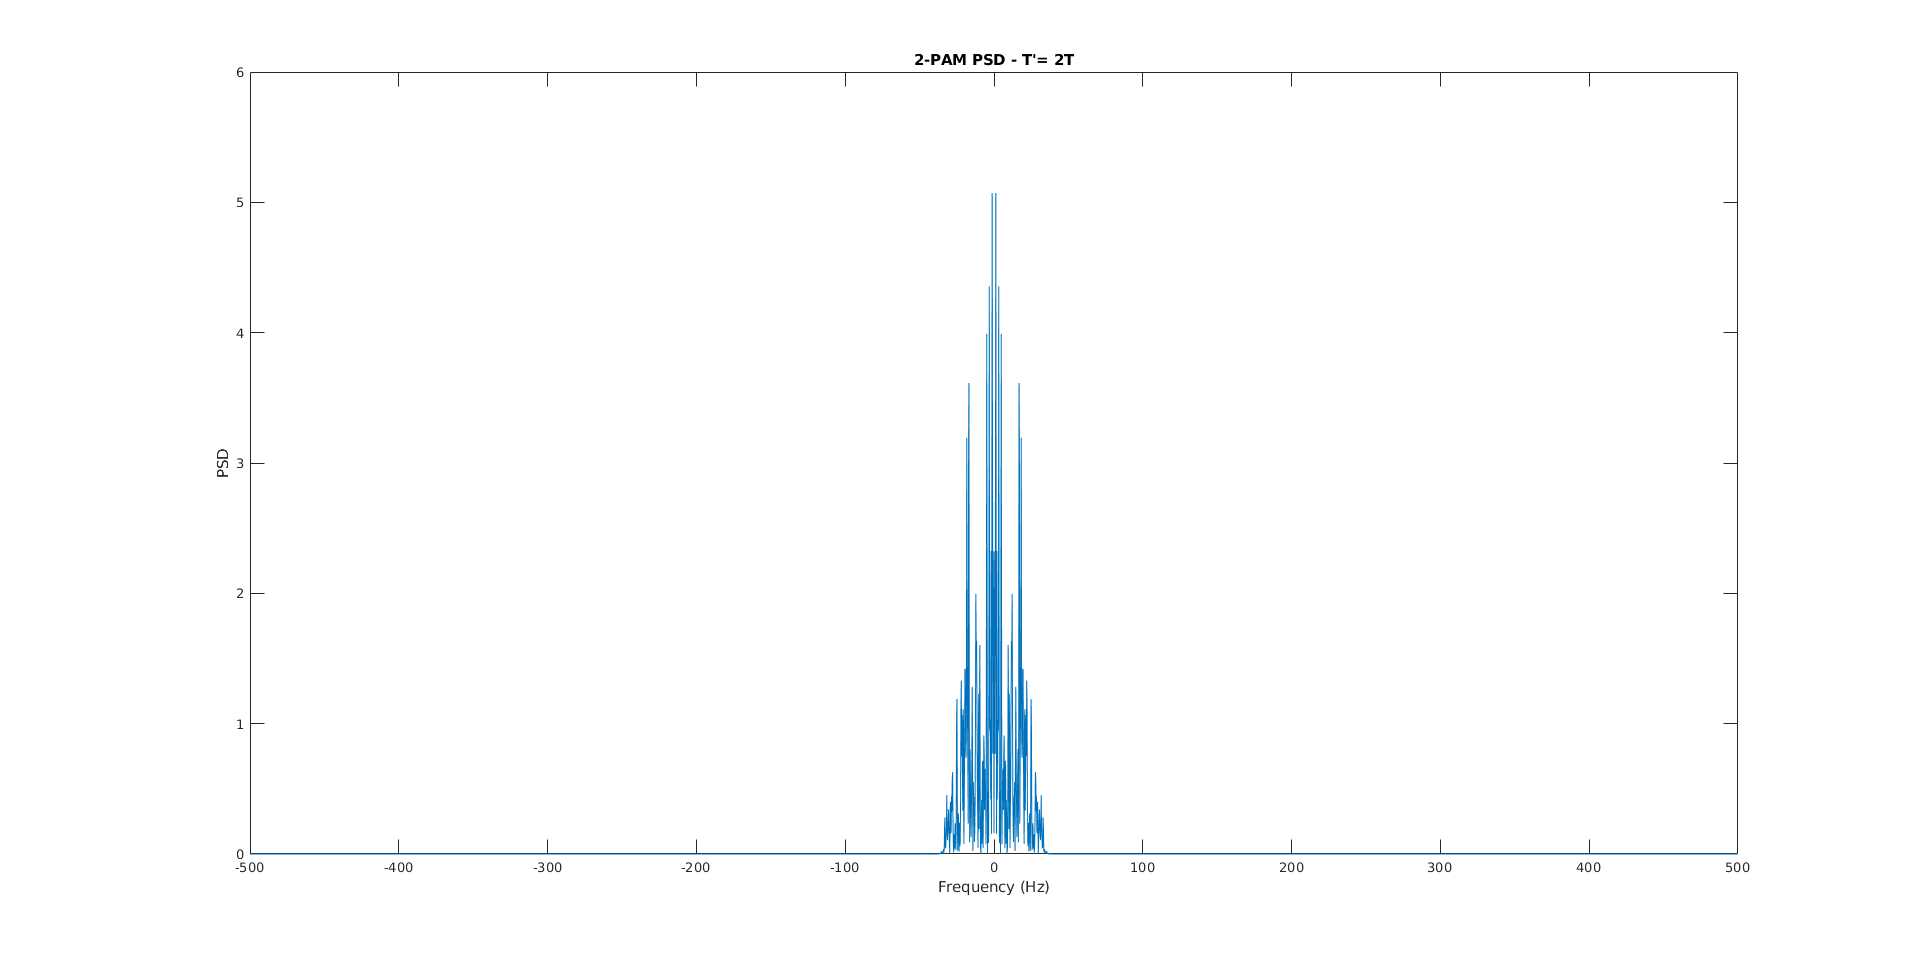
\includegraphics[width=\textwidth]{2PAM_PSD_PLOT_2T.png}
            \noindent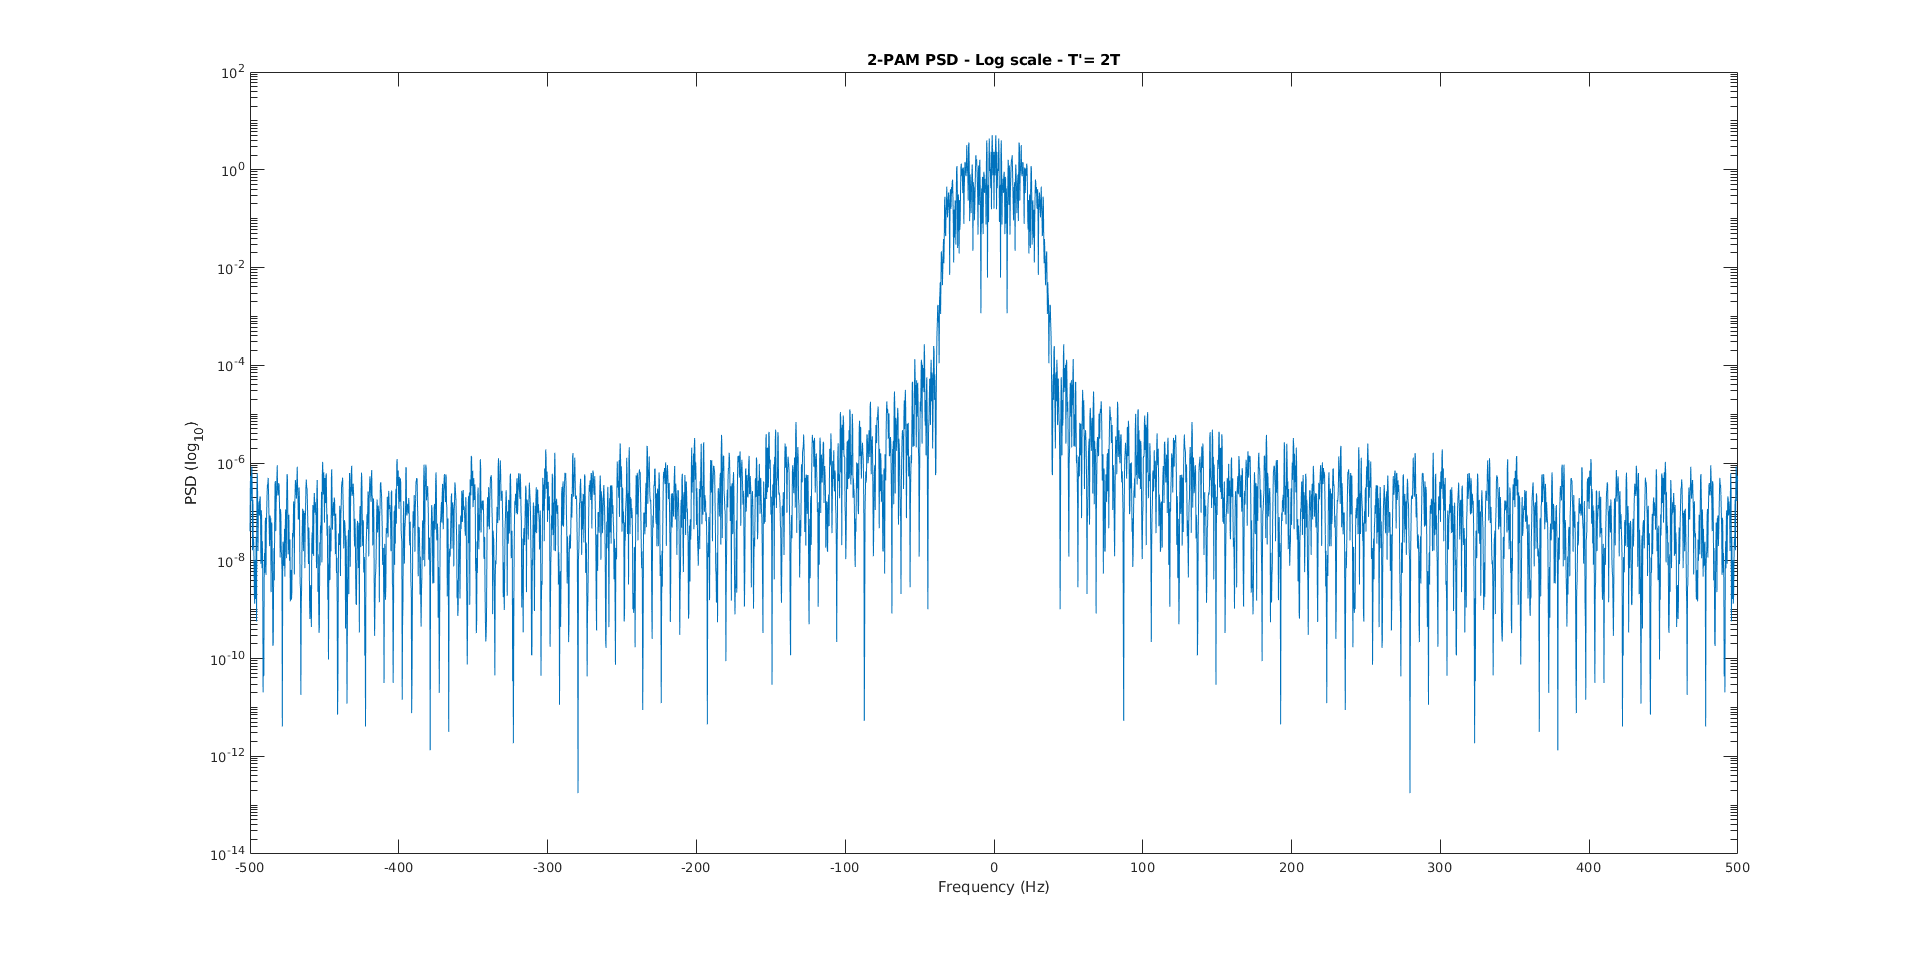
\includegraphics[width=\textwidth]{PAM_PSD_2T.png}
            \caption{Plot and Semilogarithmic Plot of PSD for \(T' = 2T\)}
        \end{figure}
        We can observe that the Bandwidth is halved from the previous signals. This is the result of the equation:
        \[BW = \frac{1+a}{2T}\]
        Doubling the Period halves the BW.\
        \begin{figure}[H]
            \centering
            \noindent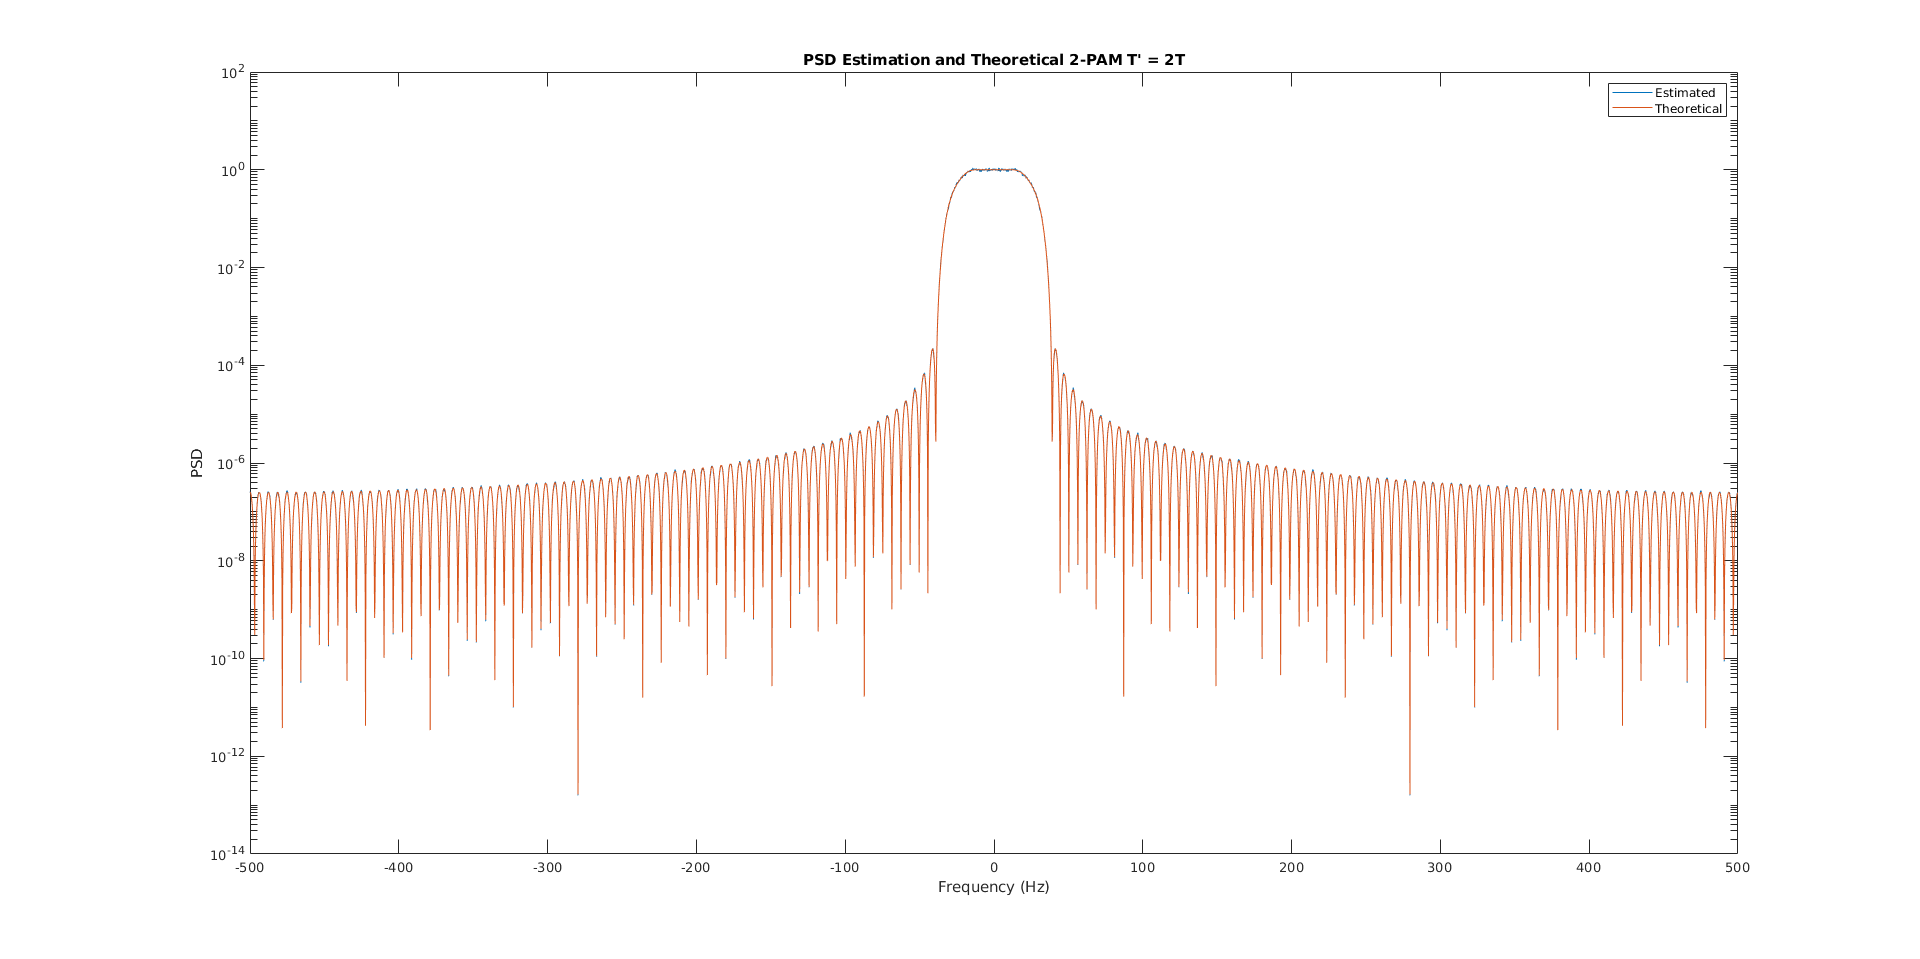
\includegraphics[width=\textwidth]{PSD_EST_THE_2T.png}
            \caption{Theoretical and Estimated graphs of the PSD of the signal \(X(t)\)}
        \end{figure}
        \item[A.6]
        \begin{itemize}
            \item If we want to send data as fast as possible, we'd most likely use a 4-PAM signal because it transfers twice the data in the same time.
            \item If the available BW is expensive then we should double the period \(T\) in order to reduce the bandwidth.
        \end{itemize}
    \end{enumerate}
	\item[B] Analyzing and confirming a theoretical problem: 
	\begin{enumerate}
		\item[B.1] Calculate \( E[Y(t)] ,\  E[Y(t + \tau)Y(t)]\):
		\[ E[Y(t)] = E[X(t) \cdot cos(2\pi f_0 t + \Theta)] = E[X(t)] \cdot E[cos(2\pi f_0 t + \Theta)] \]
			\(\Theta\) is a uniformly distributed random variable with a probability density function:
		\[f_{\Theta}(\theta) = \begin{cases} 
			\frac{1}{2\pi}, & 0 \le \theta < 2\pi \\
			0, & \text{otherwise}
		\end{cases}
		\]
		\[E[X(t)] = E\left[\sum_{n = -\infty}^{\infty} X_n \cdot \phi (t-nT)  \right] = \sum_{n=-\infty}^{\infty}E[X_n] \cdot \phi(t-nT) \]
		\[E[X_n] = 0 \Rightarrow \boxed{E[Y(t)] = 0}\]
		\[E[Y(t + \tau)Y(t)] = R_{yy}(t + \tau, t)\]
		\[= E[X(t +\tau) cos(2\pi f_0(t+ \tau) + \Theta) X(t) cos(2\pi f_0t + \Theta)]\]
		\[= E[X(t+\tau) X(t)]\cdot E[cos(2\pi f_0(t+\tau) + \Theta)cos(2\pi f_0 t + \Theta)]\star\]
		\[= E[X(t+\tau) X(t)]\cdot \frac{1}{2}E[\cancelto{0}{cos(4\pi f_0t+2\pi f_0 \tau + 2\Theta)} + cos(2 \pi f_0 \tau)] \star\star\]
		\[= \boxed{\frac{1}{2} R_{xx}(t+\tau,t) cos(2\pi f_0 \tau)}\]
		
		\[\star cos(a)cos(b) = \frac{1}{2}(cos(a+b)+cos(a-b))\]
		\[\star\star E[cos(4\pi f_0t+2\pi f_0 \tau + 2\Theta)] = \int_{0}^{2\pi}cos(4\pi f_0t+2\pi f_0 \tau + 2\theta)\cdot f_{\Theta}(\theta)\cdot d\theta = 0\]
		\item[B.2] Classify \(Y(t)\) as per its cyclostationarity:
		\[R_{xx}(t+\tau , t) = E[X(t+\tau)X(t)] = E\left[\sum_{n=-\infty}^{\infty} X_n\phi(t+\tau-nT) \cdot \sum_{n=-\infty}^{\infty} X_n\phi(t-nT)\right]\]
		\[= \sum_{n=-\infty}^{\infty} E[X_n^2] \phi(t + \tau -nT)\phi(t-nT)\]
		\[ = \sigma_X^2 \sum_{n=-\infty}^{\infty} \phi(t + \tau -nT)\phi(t-nT)\]
		\[ = \boxed{R_{xx}(t+\tau+T, t+T), \text{Cyclostationary}}\]
		\[\therefore\]
		\[\boxed{R_{yy}(t+\tau+T, t+T) = \frac{1}{2}R_{xx}(t+\tau +T,t+T)\cdot cos(2\pi f_0\tau)}\]
		\begin{center}
			 Y(t) is Cyclostationary, in the wide-sense
		\end{center}
		\item[B.3] Calculate the PSD of \(Y(t)\) (\(S_Y(F)\)) in terms of \(S_x(F)\) and \(f_0\):\\
		Since we proved that \(Y(t)\) is Cyclostationary then the following holds:
		\[S_Y(F) = F[\bar{R}_Y(\tau)]\]
		\[\bar{R}_Y(\tau) = \frac{1}{T}\int_{T}R_{yy}(t+\tau,t)dt\]
		\[=  \frac{1}{2T}\int_{0}^{T} R_{xx}(t+\tau,t)\cdot cos(2\pi f_0 \tau) dt\]
		\[ = \frac{1}{2}cos(2\pi f_0 \tau)\bar{R}_X(\tau)\]
		\[S_Y(F) = F\left[\frac{1}{2}cos(2\pi f_0 \tau)\bar{R}_X(\tau)\right]\]
		\[S_Y(F) = \frac{1}{2}F\left[cos(2\pi f_0 \tau)\bar{R}_X(\tau)\right]\]
		\[\boxed{S_Y(F) = \frac{1}{4}(S_X(F-f_0) + S_X(F+f_0))}\]
		\item[B.4] To confirm the above equation:\\
		Code for creating the average \(S_Y(F))\)
		\begin{lstlisting}[language=MATLAB]
T = T/2;
fo = 3/(2*T);
over = over/2;

[phi, phi_t] = srrc_pulse(T, over, A, a);

for i=1:500
theta = 2*pi*rand();
[X_t_t,X_t,dur] = modulate_2PAM(phi_t, phi, N_bits, Ts, over);
y_t = X_t.*cos(2*pi*fo*X_t_t + theta);
Pxf_table(i,:) = abs(fftshift(fft(y_t,N_FFT)*Ts)).^2/dur;
end
		\end{lstlisting}
		\begin{enumerate}
			\item[i.] Set the frequency \(f_0\) at an arbitrary value, in our case we chose \(150 Hz\) (\(\frac{1}{2T} < f_0 < \frac{F_s}{2} - \frac{1}{2T}\))
			\item[ii.] In a loop (500 times) create a random \(X(t)\) 2-PAM signal and modulate it with \(cos(2\pi f_0t + \Theta)\) where \(\Theta\) is a random phase angle with a PDF described in B.1
			\item[iii.]	Calculate the Periodogram using the equation from A.3 and append it to a table 
			\item[iv.] After exiting the loop average out the table from above to derive the PSD
			\item[v.] Plot the PSD and we should have spikes centered at the selected \(f_0\ and\ -f_0\) just as we proved in B.3
		\end{enumerate}
		 \begin{figure}[H]
			\centering
			\noindent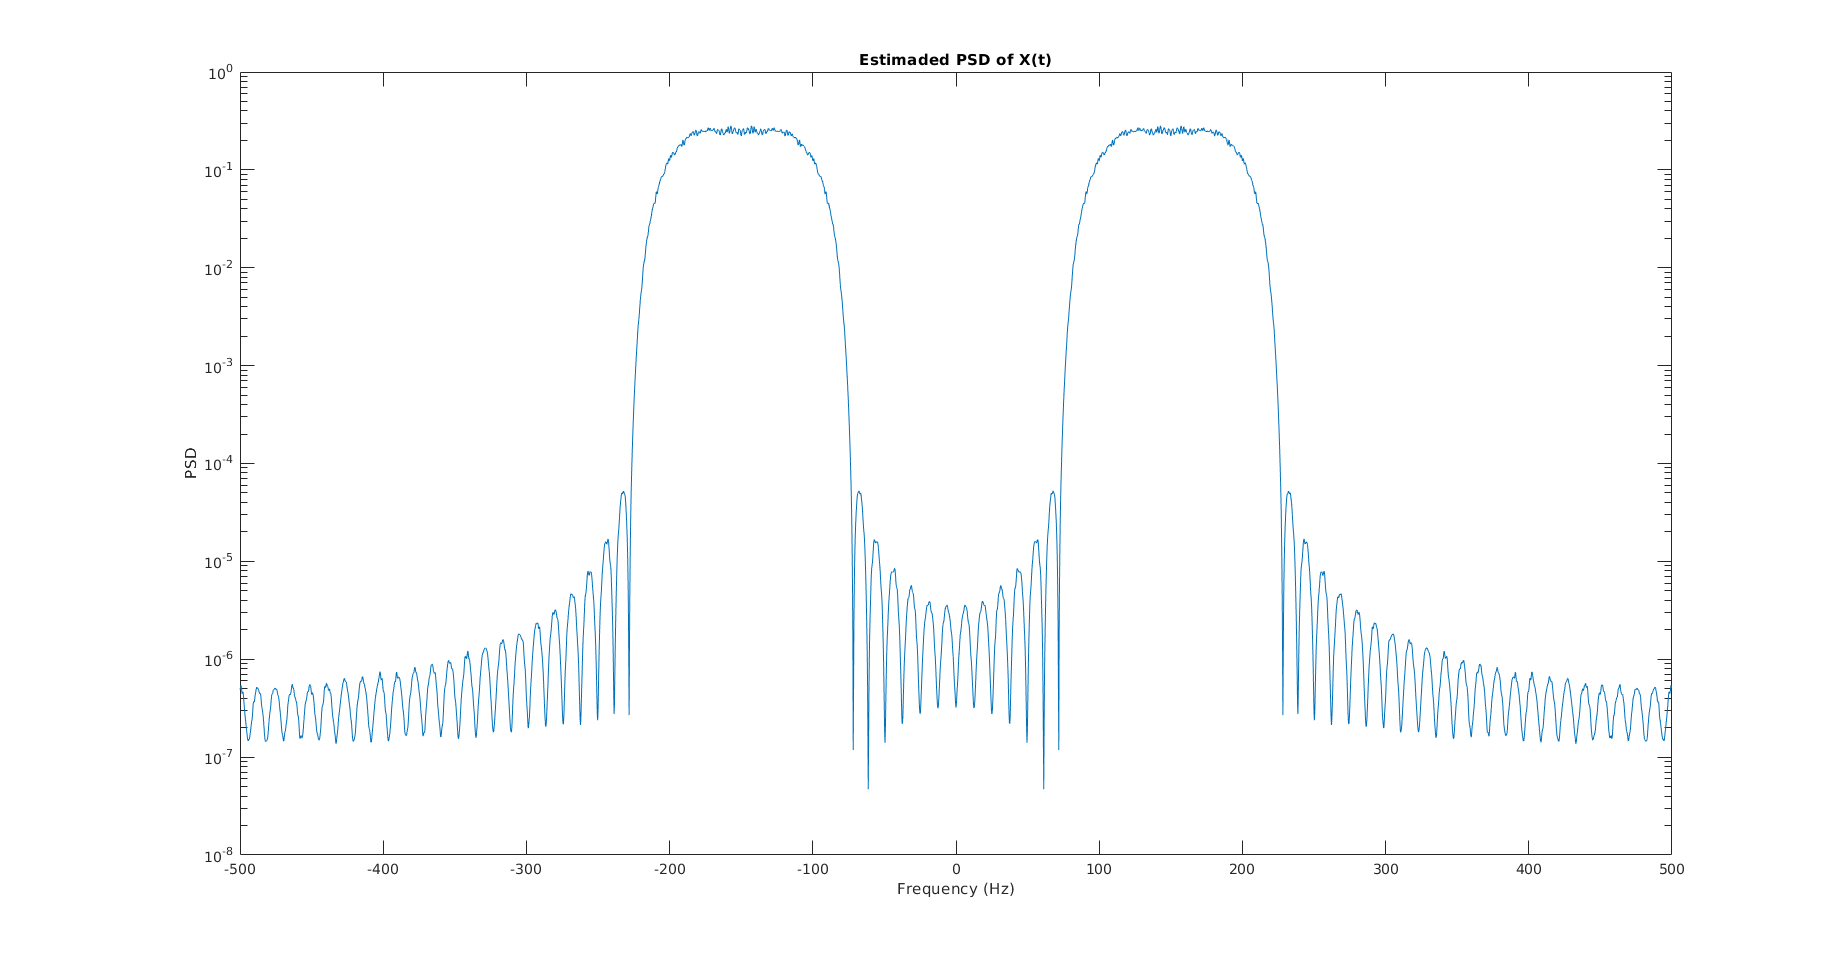
\includegraphics[width=\textwidth]{RAND_PSD.png}
			\caption{Power spikes at \(f_0\) and \(-f_0\)}
		\end{figure}
	\end{enumerate}
\end{enumerate}

\end{document}